\documentclass[11pt]{article}

% Packages
\usepackage[colorlinks]{hyperref}
\usepackage{listings}
\usepackage{graphicx}
\usepackage[dvipsnames]{xcolor}
\usepackage{amsmath}

% Colors
\definecolor{mygray}{RGB}{235,235,235}

% Margins
\setlength{\topmargin}{-2cm}
\setlength{\textwidth}{16.5cm}
\setlength{\textheight}{24cm}
\setlength{\evensidemargin}{0cm}
\setlength{\oddsidemargin}{0cm}

% Fix link colors
\hypersetup{
    colorlinks = true,
    linkcolor=red,
    citecolor=red,
    urlcolor=blue,
    linktocpage % so that page numbers are clickable in toc
}


% Code listings
\lstset{
  basicstyle=\ttfamily,
  keywordstyle=\color{blue}\ttfamily,
  stringstyle=\color{red}\ttfamily,
  commentstyle=\color{magenta}\ttfamily,
  morecomment=[l][\color{magenta}]{\#}
}


\lstnewenvironment{cli}
                  {\footnotesize
                    \lstset{columns=fullflexible,
                      language=bash,
                      backgroundcolor=\color{mygray}
                  }}
{}

\lstnewenvironment{xml}
                  {\footnotesize
                    \lstset{columns=fullflexible,
                      language=XML,
                      backgroundcolor=\color{Salmon},
                      morekeywords={property,name,value,description,configuration}
                  }}
{}

\newcommand{\bashcode}[1]{
  \begin{footnotesize}
  \par
  \hfill \colorbox{SkyBlue}
         {
           \href{https://github.com/glatard/big-data-analytics-labs/raw/master/labs/#1}
                {(\underline{Link to file})
         }} \hfill
         \lstset{language=bash,
           columns=fullflexible,
           backgroundcolor=\color{SkyBlue}}
  \vspace*{-0.3cm}
  \lstinputlisting{#1}
  \end{footnotesize}
}

\newcommand{\javacode}[1]{
  \begin{footnotesize}
  \par
  \hfill \colorbox{YellowGreen}
         {\href{https://github.com/glatard/big-data-analytics-labs/raw/master/labs/#1}
           {(\underline{Link to file})
         }} \hfill
         \lstset{language=java,
           columns=fullflexible,
           backgroundcolor=\color{YellowGreen}}
  \vspace*{-0.3cm}
%  \lstinputlisting{#1}
  \end{footnotesize}
}

\newcommand{\textfile}[1]{
  \begin{footnotesize}
  \par
  \hfill \colorbox{SkyBlue}
         {\href{https://github.com/glatard/big-data-analytics-labs/raw/master/labs/#1}
           {(\underline{Link to file})
         }} \hfill
         \lstset{columns=fullflexible,
           backgroundcolor=\color{SkyBlue}}
  \vspace*{-0.3cm}
  \lstinputlisting{#1}
  \end{footnotesize}
}


% Notes and TODOs              
\newcommand{\postit}[1]{%
%  \noindent
%  \fcolorbox{red}{yellow}{%
%    \begin{minipage}{5cm}
%      #1
%    \end{minipage}
%   }
}

\title{\textsc{Big Data Analytics (SOEN 498/691)} \\ Laboratory sessions}

\author{Tristan Glatard\\Department of Computer Science and Software Engineering\\Concordia University, Montreal\\\href{mailto:tristan.glatard@concordia.ca}{tristan.glatard@concordia.ca}}

\begin{document}

\maketitle

\newpage

\tableofcontents

\newpage

\part{k-means}

\section{Introduction}

Clustering is a technique used in a variety of applications to
categorize elements of a data set. We will implement the k-means
clustering algorithm in MapReduce. k-means is a very popular
clustering algorithm due to its simplicity.

Given a dataset consisting of $n$ elements and an integer $k\leq n$, the algorithm works as follows:
\begin{enumerate}
\item Initialization: select $k$ initial means $m_1$, ... , $m_k$. Means are also called centroids.
\item Assignment: assign every element $x$ of the dataset to a set
  $S_i$ such that $i=\mathrm{argmin}_{i \in [\![1,k]\!]}(d(x,m_i))$,
  where $d(.,.)$ is a distance in the data set.
\item Update: update $m_i$ as the mean of the elements in $S_i$.
\end{enumerate}
Repeat steps 2 and 3 until the $m_i$ no longer change.

FIgure~\ref{fig:illustration} illustrates the input and output of the
k-means algorithm on a dataset of 1,000 points clustered in 4 clusters.
\begin{figure}[h]
  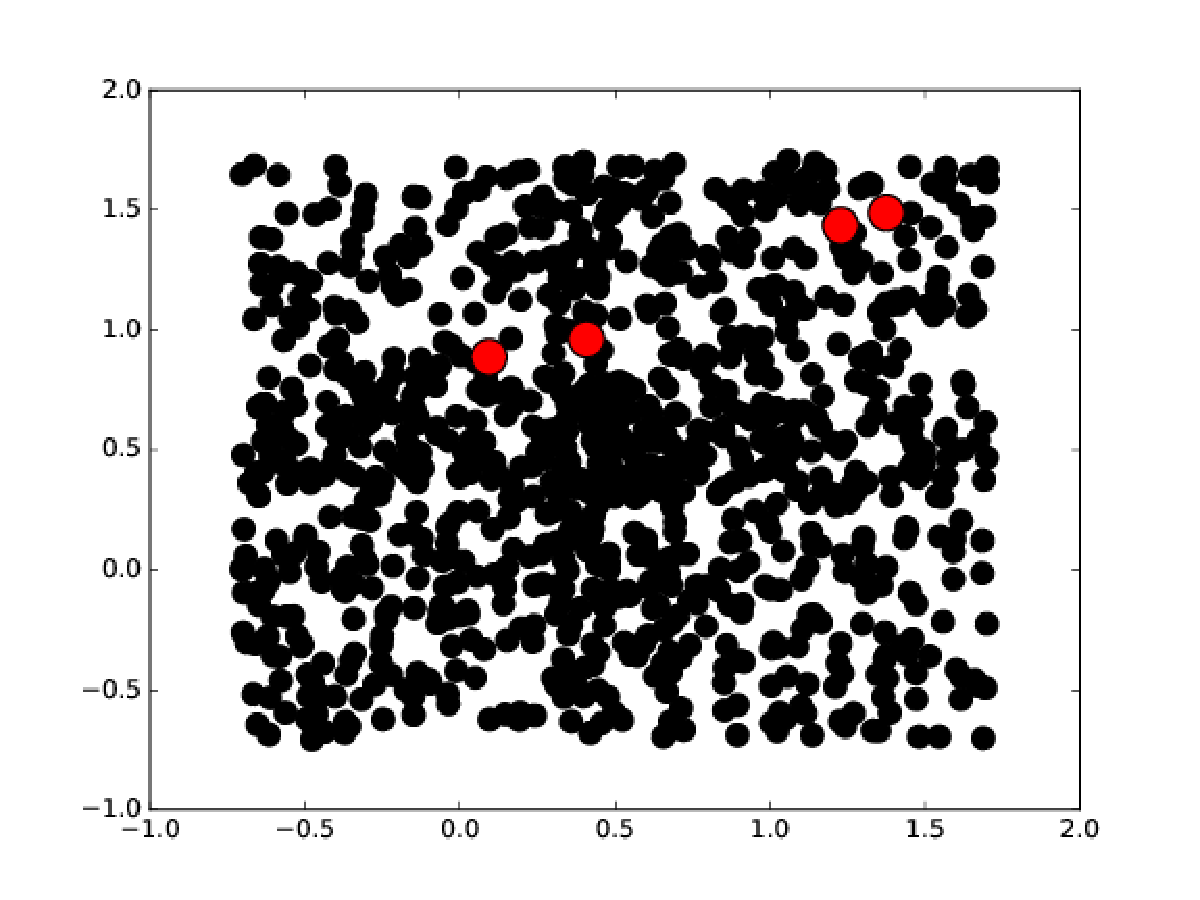
\includegraphics[width=0.5\textwidth]{kmeans/initialisation.pdf}
  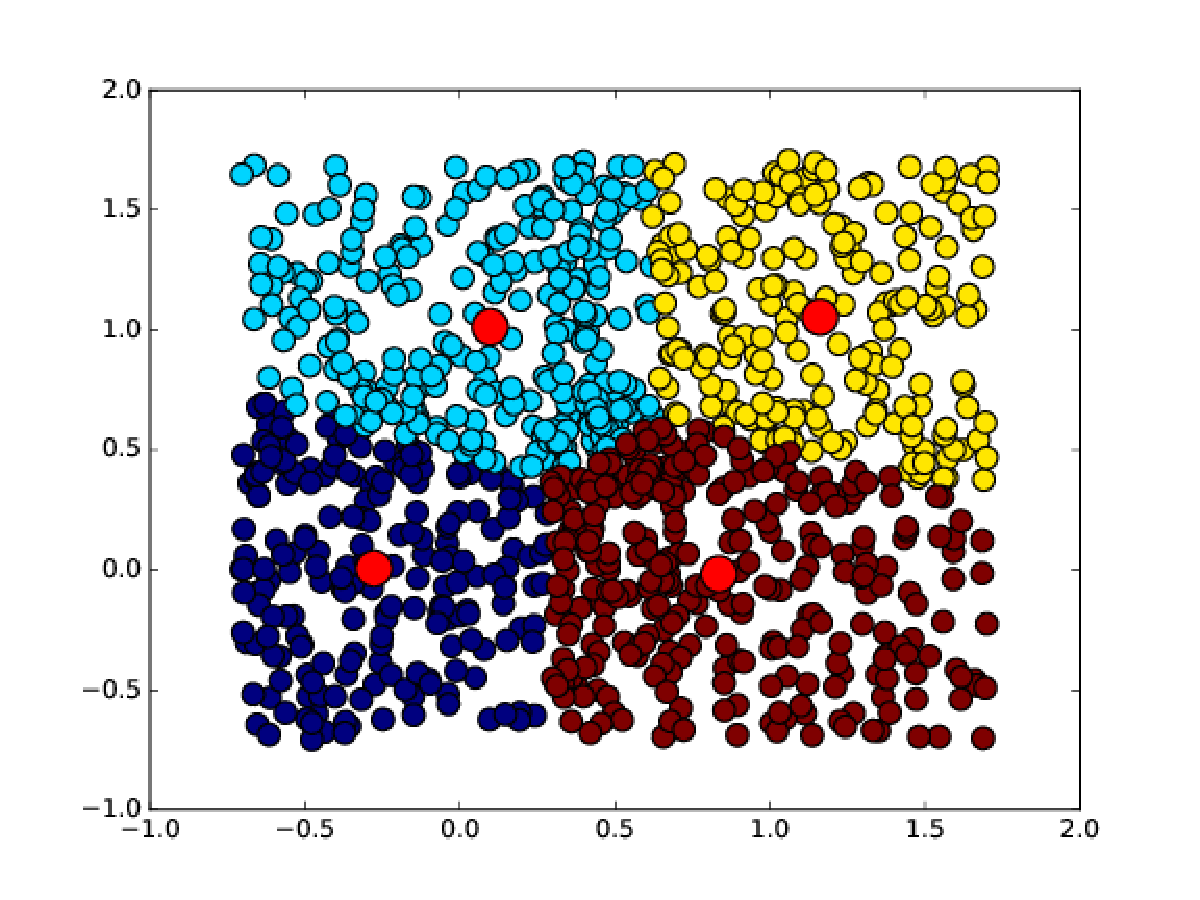
\includegraphics[width=0.5\textwidth]{kmeans/converged.pdf}
  \label{fig:illustration}
  \caption{Illustration of k-means algorithm. Left: input dataset
    (black) and centroid initialization (red). Right: classification
    (the 4 different clusters are represented in cyan, blue, yellow and brown) and
    final centroid locations (red).}
\end{figure}

\section{Basic idea}

We focus on a dataset containing 2D points. We will implement each
iteration of the k-means algorithm as a MapReduce job.
\begin{itemize}
\item Map step:
  \begin{itemize}
  \item Receive (\_,v): \_, (\texttt{x},\texttt{y}) \newline
    where \texttt{x} and \texttt{y} are the coordinates of a point in the dataset.
  \item Emit (k,v): \texttt{i}, (\texttt{x},\texttt{y}) \newline
    where \texttt{i} is the index of the closest centroid to (\texttt{x},\texttt{y}).
  \end{itemize}
\item Reduce step:
  \begin{itemize}
  \item Receive (k, [v]): \texttt{i}, [(\texttt{x$_1$},\texttt{y$_1$}), (\texttt{x$_2$},\texttt{y$_2$}), \ldots]
  \item Emit (k,v): \texttt{i}, (\texttt{$\bar x$}, \texttt{$\bar y$}) \newline
    where \texttt{$\bar x$} and \texttt{$\bar y$} are the means of the \texttt{x$_i$} and \texttt{y$_i$}, respectively.
  \end{itemize}
\end{itemize}
The centroids will be written in a file distributed to the mappers
through the distributed cache. Convergence of the algorithm will be
detected when the hash of this file no longer changes. Every iteration
will produce a list of $k$ centroids. Once the algorithm converged, a
final map job will be run to output the classification.

% Without and with a combiner.

\section{Implementation}


\end{document}


